%----------------------------------------------------------------------------------------
%	PACKAGES AND OTHER DOCUMENT CONFIGURATIONS
%----------------------------------------------------------------------------------------

\documentclass[
    12pt,
%oneside, % Two side (alternating margins) for binding by default, uncomment to switch to one side
    english, % ngerman for German
    singlespacing, % Single line spacing, alternatives: onehalfspacing or doublespacing
%draft, % Uncomment to enable draft mode (no pictures, no links, overfull hboxes indicated)
%nolistspacing, % If the document is onehalfspacing or doublespacing, uncomment this to set spacing in lists to single
%liststotoc, % Uncomment to add the list of figures/tables/etc to the table of contents
%toctotoc, % Uncomment to add the main table of contents to the table of contents
%parskip, % Uncomment to add space between paragraphs
%nohyperref, % Uncomment to not load the hyperref package
%headsepline, % Uncomment to get a line under the header
%chapterinoneline, % Uncomment to place the chapter title next to the number on one line
%consistentlayout, % Uncomment to change the layout of the declaration, abstract and acknowledgements pages to match the default layout
    oneside, % uncomment for clear page spacing between sections
]{MastersDoctoralThesis} % The class file specifying the document structure

\usepackage[utf8]{inputenc} % Required for inputting international characters
\usepackage[T1]{fontenc} % Output font encoding for international characters
\usepackage{newtxmath,newtxtext}
\usepackage{float}% If comment this, figure moves to Page 2
\usepackage{spverbatim}

\usepackage{mathpazo} % Use the Palatino font by default

\usepackage[backend=bibtex,style=authoryear,natbib=true]{biblatex} % Use the bibtex backend with the authoryear citation style (which resembles APA)

\addbibresource{main.bib} % The filename of the bibliography

\usepackage[autostyle=true]{csquotes}
\usepackage{amsmath}
\usepackage{bm} % Required to generate language-dependent quotes in the bibliography
\usepackage{eso-pic}


% adds header image to each page
%\AddToShipoutPictureBG{
%    \AtPageUpperLeft{
%        \raisebox{-2\height}{
%            \hspace*{6.0cm}
\includegraphics[height=1.2cm]{Pictures/wsb_logo}
%        }
%    }
%}
%----------------------------------------------------------------------------------------
%	MARGIN SETTINGS
%----------------------------------------------------------------------------------------

\geometry{
    paper=a4paper, % Change to letterpaper for US letter
    inner=2.5cm, % Inner margin
    outer=3.8cm, % Outer margin
    bindingoffset=.5cm, % Binding offset
    top=1.5cm, % Top margin
    bottom=1.5cm, % Bottom margin
    headheight = 3.5cm
%showframe, % Uncomment to show how the type block is set on the page
}

%----------------------------------------------------------------------------------------
%	THESIS INFORMATION
%----------------------------------------------------------------------------------------

\thesistitle{The Mango Messenger} % Your thesis title, this is used in the title and abstract, print it elsewhere with \ttitle
\supervisor{Dr. Szymon Murawski} % Your supervisor's name, this is used in the title page, print it elsewhere with \supname
\examiner{} % Your examiner's name, this is not currently used anywhere in the template, print it elsewhere with \examname
\degree{Bachelor of Computer Science} % Your degree name, this is used in the title page and abstract, print it elsewhere with \degreename
\author{Petro Kolosov, Serhii Holishevskyi, Illia Zubachov, Arslanbek Temirbekov} % Your name, this is used in the title page and abstract, print it elsewhere with \authorname
\addresses{} % Your address, this is not currently used anywhere in the template, print it elsewhere with \addressname

\subject{Biological Sciences} % Your subject area, this is not currently used anywhere in the template, print it elsewhere with \subjectname
\keywords{} % Keywords for your thesis, this is not currently used anywhere in the template, print it elsewhere with \keywordnames
\university{Wyzsza Szkola Bankowa w Poznaniu} % Your university's name and URL, this is used in the title page and abstract, print it elsewhere with \univname
\department{Department of Computer Science} % Your department's name and URL, this is used in the title page and abstract, print it elsewhere with \deptname
\group{Wyzsza Szkola Bankowa w Poznaniu} % Your research group's name and URL, this is used in the title page, print it elsewhere with \groupname
\faculty{Computer Science} % Your faculty's name and URL, this is used in the title page and abstract, print it elsewhere with \facname

\AtBeginDocument{
    \hypersetup{pdftitle=\ttitle} % Set the PDF's title to your title
    \hypersetup{pdfauthor=\authorname} % Set the PDF's author to your name
    \hypersetup{pdfkeywords=\keywordnames} % Set the PDF's keywords to your keywords
}

\pagestyle{myheadings}
\ohead*{}\ofoot*{\pagemark}

\begin{document}

    \frontmatter % Use roman page numbering style (i, ii, iii, iv...) for the pre-content pages

    %\pagestyle{myheadings} % Default to the plain heading style until the thesis style is called for the body content

%----------------------------------------------------------------------------------------
%	TITLE PAGE
%----------------------------------------------------------------------------------------
    \begin{titlepage}
        \begin{center}
%            
\includegraphics[width=0.5\textwidth]{Pictures/wsb_logo} \\ % University/department logo - uncomment to place it
%            \vspace*{.06\textheight}
%        {\scshape\LARGE \univname\par}
            %\vspace{1.5cm} % University name
            \textsc{DEPARTMENT OF COMPUTER SCIENCE}\\[0.5cm] % Thesis type

            %\HRule \\[0.4cm] % Horizontal line
            \vspace{3cm}
            {\huge \bfseries \ttitle\par}
            \vspace{0.4cm}
            %\HRule \\[1.5cm] % Horizontal line

%            \begin{minipage}[t]{0.4\textwidth}
%                \begin{flushleft}
%                    \large
%                    \emph{Authors:}\\
%                    \authorname % Author name - remove the \href bracket to remove the link
%                \end{flushleft}
%            \end{minipage}
%            \begin{minipage}[t]{0.4\textwidth}
%                \begin{flushright}
%                    \large
%                    \emph{Supervisor:} \\
%                    \supname % Supervisor name - remove the \href bracket to remove the link
%                \end{flushright}
%            \end{minipage}\\[3cm]

            \vfill
            \textsc{\Large DIPLOMA PROJECT}\\[0.5cm]

%            \large \textit{A thesis submitted in fulfillment of the requirements\\ for the degree of \degreename}\\[0.3cm] % University requirement text
%            \textit{in the}\\[0.4cm]
%            \groupname\\\deptname\\[2cm] % Research group name and department name

%            \vfill

            \vspace*{\fill}
            {\large Poznan, \the\year{}}

%            \vfill
        \end{center}
    \end{titlepage}

%----------------------------------------------------------------------------------------
%	DECLARATION PAGE
%----------------------------------------------------------------------------------------

%    \begin{declaration}
%        \addchaptertocentry{\authorshipname} % Add the declaration to the table of contents
%        \noindent We, \authorname, declare that this thesis titled, \enquote{\ttitle} and the work
%        presented in it are our own.
%        We confirm that:
%
%        \begin{itemize}
%            \item This work was done wholly or mainly while in candidature for a research degree at WSB in Poznan University.
%            \item Where any part of this thesis has previously been submitted for a degree or any other qualification
%            at this University or any other institution, this has been clearly stated.
%            \item Where We have consulted the published work of others, this is always clearly attributed.
%            \item Where We have quoted from the work of others, the source is always given.
%            With the exception of such quotations, this thesis is entirely our own work.
%            \item We have acknowledged all main sources of help.
%            \item Where the thesis is based on work done by ourselves jointly with others,
%            We have made clear exactly what was done by others and what I have contributed myself.\\
%        \end{itemize}
%
%        \noindent Signed: \\
%        \rule[0.5em]{25em}{0.5pt} % This prints a line for the signature
%
%        \noindent Date: \\
%        \rule[0.5em]{25em}{0.5pt} % This prints a line to write the date
%    \end{declaration}

%----------------------------------------------------------------------------------------
%	PARTNER DETAILS PAGE
%---------------------------------------------------------------------------------------


    \section*{Partner Details}\label{sec:partner-details}
    \begin{description}
        \item \hspace*{8mm}\textbf{Mentor's details} \\

        \begin{tabular}{|p{0.5\textwidth}|p{0.5\textwidth}|}
            \hline
            First name and surname & Szymon Murawski \\
            \hline
            Degree                 & Dr. Inz.        \\
            \hline
            Date and signature     &                 \\
            \hline
            \multicolumn{2}{c}{\vspace{0.5cm}} \\
        \end{tabular}
        \item \hspace*{8mm}\textbf{Team members' details} \\

        \begin{tabular}{|p{0.5\textwidth}|p{0.5\textwidth}|}
            \hline
            First name and surname & Petro Kolosov        \\
            \hline
            Course of study        & Computer Science     \\
            \hline
            Type of study program  & Daytime              \\
            \hline
            Date and signature     &                      \\
            \hline

            \multicolumn{2}{c}{\vspace{0.5cm}} \\

            \hline
            First name and surname & Serhii Holishevskyi  \\
            \hline
            Course of study        & Computer Science     \\
            \hline
            Type of study program  & Daytime              \\
            \hline
            Date and signature     &                      \\
            \hline

            \multicolumn{2}{c}{\vspace{0.5cm}} \\

            \hline
            First name and surname & Illia Zubachov       \\
            \hline
            Course of study        & Computer Science     \\
            \hline
            Type of study program  & Daytime              \\
            \hline
            Date and signature     &                      \\
            \hline

            \multicolumn{2}{c}{\vspace{0.5cm}} \\

            \hline
            First name and surname & Arslanbek Temirbekov \\
            \hline
            Course of study        & Computer Science     \\
            \hline
            Type of study program  & Daytime              \\
            \hline
            Date and signature     &                      \\
            \hline
        \end{tabular}
    \end{description}

%----------------------------------------------------------------------------------------
%	QUOTATION PAGE
%----------------------------------------------------------------------------------------

%    \vspace*{0.2\textheight}
%
%    \noindent\enquote{\itshape
%    I fear not the man who has practiced 10,000 kicks once, but I fear the man who has practiced one kick 10,000 times.}\bigbreak
%
%    \hfill Bruce Lee

%----------------------------------------------------------------------------------------
%	ABSTRACT PAGE
%----------------------------------------------------------------------------------------

%    \begin{abstract}
%        \addchaptertocentry{\abstractname} % Add the abstract to the table of contents
%        Nowadays, instant messaging systems achieve a great success and became the main mean of communication
%        between people via an internet.
%        Thanks to the simplicity and quickness of the message exchanging more and more people over the world start to use
%        instant messengers on daily basis.
%        However, such a great attention forces us to discuss another aspect of these systems, an aspect of the
%        information security and user privacy.
%        The main aim of this thesis is to design and implement an instant messaging system
%        that copes with the required functionalities and satisfies the defined security requirements.
%    \end{abstract}

%----------------------------------------------------------------------------------------
%	ACKNOWLEDGEMENTS
%----------------------------------------------------------------------------------------

%    \begin{acknowledgements}
%        \addchaptertocentry{\acknowledgementname} % Add the acknowledgements to the table of contents
%        We would like to thank our mentor Szymon Murawski for his useful comments and suggestions and support
%        over the whole process of writing this thesis.
%    \end{acknowledgements}

%----------------------------------------------------------------------------------------
%	LIST OF CONTENTS/FIGURES/TABLES PAGES
%----------------------------------------------------------------------------------------

    \tableofcontents % Prints the main table of contents
%
%    \listoffigures % Prints the list of figures
%
%    \listoftables % Prints the list of tables

%----------------------------------------------------------------------------------------
%	ABBREVIATIONS
%----------------------------------------------------------------------------------------

%    \begin{abbreviations}{ll} % Include a list of abbreviations (a table of two columns)
%
%        \textbf{HTTP} & Hypertext Transfer Protocol \\
%        \textbf{DoS} & Denial of Service \\
%        \textbf{DDoS} & Distributed Denial of Service \\
%        \textbf{XSRF, CSRF} & Cross-site request forgery \\
%        \textbf{XSS} & Cross-site scripting \\
%        \textbf{GRASP} & General Responsibility Assignment Software Patterns \\
%        \textbf{API} & Application Programming Interface \\
%        \textbf{IPC} & Institute of Printed Circuits \\
%        \textbf{CQRS} & Command Query Responsibility Segregation\\
%        \textbf{CRUD} & Create Read Update Delete\\
%        \textbf{UUID} & Universally unique identifier \\
%        \textbf{GUID} & Globally Unique Identifier \\
%        \textbf{JSON} & JavaScript Object Notation \\
%        \textbf{JWT} & JSON Web Token \\
%        \textbf{RFC} & Request for Comments \\
%        \textbf{RSA} & Rivest-Shamir-Adleman \\
%        \textbf{HMAC} & Hash-Based Message Authentication Codes \\
%        \textbf{ECDSA} & Elliptic Curve Digital Signature Algorithm \\
%        \textbf{HTTPS} & Hypertext Transfer Protocol Secure \\
%        \textbf{TLS} & Transport Layer Security \\
%        \textbf{SSL} & Secure Sockets Layer \\
%        \textbf{E2E} & End-to-End \\
%        \textbf{EDH, DHE} & Elliptic-curve Diffie–Hellman \\
%        \textbf{AES} & Advanced Encryption Standard \\
%
%    \end{abbreviations}

%----------------------------------------------------------------------------------------
%	PHYSICAL CONSTANTS/OTHER DEFINITIONS
%----------------------------------------------------------------------------------------

%    \begin{constants}{lr@{${}={}$}l} % The list of physical constants is a three column table
%
%    % The \SI{}{} command is provided by the siunitx package, see its documentation for instructions on how to use it
%
%        Speed of Light & $c_{0}$ & \SI{2.99792458e8}{\meter\per\second} (exact)\\
%    %Constant Name & $Symbol$ & $Constant Value$ with units\\
%
%    \end{constants}

%----------------------------------------------------------------------------------------
%	SYMBOLS
%----------------------------------------------------------------------------------------

%    \begin{symbols}{lll} % Include a list of Symbols (a three column table)
%
%        $a$ & distance & \si{\meter} \\
%        $P$ & power & \si{\watt} (\si{\joule\per\second}) \\
%        %Symbol & Name & Unit \\
%
%        \addlinespace % Gap to separate the Roman symbols from the Greek
%
%        $\omega$ & angular frequency & \si{\radian} \\
%
%    \end{symbols}

%----------------------------------------------------------------------------------------
%	DEDICATION
%----------------------------------------------------------------------------------------

%    \dedicatory{For/Dedicated to/To my\ldots}

%----------------------------------------------------------------------------------------
%	THESIS CONTENT - CHAPTERS
%----------------------------------------------------------------------------------------

    \mainmatter % Begin numeric (1,2,3...) page numbering

    \pagestyle{thesis} % Return the page headers back to the "thesis" style

% Include the chapters of the thesis as separate files from the Chapters folder
% Uncomment the lines as you write the chapters
    \chapter{Project Assumptions}\label{ch:project-assumptions}


\section{Project description}\label{sec:project-description}
[Please provide an abbreviated description of the project, in line with the following structure.
The description should not be more than 10,000 characters long (including spaces).
Please use Times New Roman font, 12 pts, 1.5 spacing.]
\begin{enumerate}
    \item Research project
    \item Justification for selecting the subject
    \item Project's scope in terms of subject matter, object of research, time and space
    \item Work methodology research (method and techniques)
\end{enumerate}

Nowadays, instant messaging systems achieve a great success and became the main mean of communication
between people via an internet.
Thanks to the simplicity and quickness of the message exchanging more and more people over the world start to use
instant messengers on daily basis.
However, such a great attention forces us to discuss another aspect of these systems, an aspect of the
information security and user privacy.
The main aim of this thesis is to design and implement an instant messaging system
that copes with the required functionalities and satisfies the defined security requirements.


\section{Project objectives}\label{sec:project-objectives}
\begin{enumerate}
    \item To provide the system requirements for instant messaging system, both functional and non-functional.
    \item To analyze and propose mitigations for security and user privacy vulnerabilities of the instant messaging system.
    \item To propose web service (API's) architecture that fits the requirements.
    \item To discuss an authorization mechanism that fits the requirements.
    \item To discuss and apply E2E Encryption to the system, if necessary.
    \item To implement web service.
    \item To implement web client.
    \item To implement mobile client.
    \item To implement desktop client.
\end{enumerate}
    \chapter{Impelentation}\label{ch:impelentation}


\section{Project tasks}\label{sec:project-tasks}
\begin{description}
    \item \hspace*{8mm}\textbf{Task 1.}\\[5mm]
    \begin{tabular}{|p{5cm}|p{7cm}|}
        \hline
        Task name                                                                       & \\
        \hline
        Entities involved in the fulfilment of the task (max: 5 sentences)              & \\
        \hline
        Task completion outcomes (preparation / decisions / technical / dossier, etc. ) & \\
        \hline
        Star date of task execution                                                     & \\
        \hline
        End date of task execution                                                      & \\
        \hline
    \end{tabular}
    \item \hspace*{8mm}\textbf{Task 2.}\\[5mm]
    \begin{tabular}{|p{5cm}|p{7cm}|}
        \hline
        Task name                                                                       & \\
        \hline
        Entities involved in the fulfilment of the task (max: 5 sentences)              & \\
        \hline
        Task completion outcomes (preparation / decisions / technical / dossier, etc. ) & \\
        \hline
        Star date of task execution                                                     & \\
        \hline
        End date of task execution                                                      & \\
        \hline
    \end{tabular}
    \item \hspace*{8mm}\textbf{Task 3.}\\[5mm]
    \begin{tabular}{|p{5cm}|p{7cm}|}
        \hline
        Task name                                                                       & \\
        \hline
        Entities involved in the fulfilment of the task (max: 5 sentences)              & \\
        \hline
        Task completion outcomes (preparation / decisions / technical / dossier, etc. ) & \\
        \hline
        Star date of task execution                                                     & \\
        \hline
        End date of task execution                                                      & \\
        \hline
    \end{tabular}
    \item \hspace*{8mm}\textbf{Task 4.}\\[5mm]
    \begin{tabular}{|p{5cm}|p{7cm}|}
        \hline
        Task name                                                                       & \\
        \hline
        Entities involved in the fulfilment of the task (max: 5 sentences)              & \\
        \hline
        Task completion outcomes (preparation / decisions / technical / dossier, etc. ) & \\
        \hline
        Star date of task execution                                                     & \\
        \hline
        End date of task execution                                                      & \\
        \hline
    \end{tabular}
\end{description}

%\textbf{Task 1} \\
%
%\begin{tabular}{|p{5cm}|p{7cm}|}
%    \hline
%    Task name                                                                            & \\
%    \hline
%    Entities involved in the fulfilment of the task (max: 5 sentences)                   & \\
%    \hline
%    Task completion outcomes (preparation / decisions / technical / dossier, etc. )      & \\
%    \hline
%    Star date of task execution                                                          & \\
%    \hline
%    End date of task execution                                                           & \\
%    \hline
%\end{tabular} \\
%
%\textbf{Task 2} \\
%
%\begin{tabular}{|p{5cm}|p{7cm}|}
%    \hline
%    Task name                                                                            & \\
%    \hline
%    Entities involved in the fulfilment of the task (max: 5 sentences)                   & \\
%    \hline
%    Task completion outcomes (preparation / decisions / technical / dossier, etc. )      & \\
%    \hline
%    Star date of task execution                                                          & \\
%    \hline
%    End date of task execution                                                           & \\
%    \hline
%\end{tabular}


\section{Project implementation}\label{sec:project-implementation}
[Please develop the theoretical assumptions of the project, including notes; present the empirical part of the project – research results and conclusions, as well as subject-matter description, etc.
Please present computations and calculations, if any, in annexes.
Please do not change the names of the points below.
There is no predefined structure within individual points.
Also, additional parts, forming individual points, can be enumerated according to your own concept.
The theoretical and empirical part should not exceed 50,000 characters.
Please use Times New Roman font, 12 pts, 1.5 spacing.] \\

\begin{enumerate}
    \item Theoretical assumptions
    \item Description of facts
    \item Empirical research
\end{enumerate}


\section{Project outcomes}\label{sec:project-outcomes}
[Please describe the achieved outcomes of the project.
If possible, please provide figures showing the described outcomes.
Please confront them with the objectives of the project.
This part should be between 2000 and 10,000 characters long.
Please use Times New Roman font, 12 pts, 1.5 spacing.
Full description of solutions that were worked out and project outcomes, if any, should be presented in annexes.]


\section{Usefulness of project}\label{sec:usefulness-of-project}
[Please justify how this project is useful (how the project can be used in practice).
The description should not exceed 6000 characters.
Please use Times New Roman font, 12 pts, 1.5 spacing.]


\section{Project self-evaluation}\label{sec:project-self-evaluation}
[Each of the project’s Authors describes his or her skills and competencies that were developed while working on the project and identifies issues encountered while working on the project.
If during the work on the project the team had not completed any tasks planned earlier, or omitted them altogether, please specify what were these tasks and why they had not been completed.
This part should not exceed 6000 characters.
Please use Times New Roman font, 12 pts, 1.5 spacing.]


\section{Material and bibliography used to carry out the project}\label{sec:material-and-bibliography-used-to-carry-out-the-project}
[Please enumerate sources used by the team during the work on the project (as per the applying layout, Times New Roman font, 12 pts., 1.5 spacing).]


\section{List of annexes}\label{sec:list-of-annexes}
[In this place you should list all additional documents, e.g. preprinted forms, data sets, financial statements, survey templates, diagrams,
    concepts, strategies, studies, analyses, procedures, regulations, technical documents, plans, models, etc. which significantly contributed to the project.
Please prepare all annexes in accordance with the template in place.
Please use Times New Roman font, 12 pts, 1.5 spacing.
All annexes form an integral part of the project.]


    \chapter*{System Requirements}\label{ch:system-requirements}
\addcontentsline{toc}{chapter}{System Requirements}

In previous sections we have briefly discussed Instant Messaging System, mainly from security and user privacy aspects.
Prior to software module implementation, it is essentially important to define the functionality module will obtain.
In this section we discuss functional and non-functional requirements of secure instant messaging system from customer's prospective.

Generally, there are three forms of software product requirements: business, functional, and non-functional.
Business requirements [\cite{dilworth2007creation}] typically answer how the product will address the needs of your company and its users.
They also reveal the business model of the app and what problems it can solve.
Functional requirements [\cite{malan2001functional}] are about functionalities that will be implemented in the application.
Non-functional requirements [\cite{chung2012non}] describe how these functionalities will be implemented.

\section{Functional Requirements}\label{sec:functional-requirements}
To compete with successful and commonly used instant messaging platforms, your service has to offer great functionality.
So first, let’s define the core features of a messaging app.
\begin{itemize}
    \item Registration
    \item Authentication
    \item Authorization
    \item Adding contacts
    \item Sending messages and media to individuals
    \item Creating groups
    \item Sending messages and media to groups user stories
    \item Viewing message history
    \item Profile settings
\end{itemize}
Note that Authentication [\cite{burrows1989logic}] means confirming your own identity,
whereas Authorization [\cite{fagin1978authorization}] means being allowed access to the particular part of the system.

\subsection{Registration user stories}\label{subsec:registration}
\begin{itemize}
    \item As an unregistered user, I want to tap “register” so that I can see the registration form.
    \item As an unregistered user, I want to use my phone number to register so that my account is tied to my phone number.
    \item As an unregistered user, I want to use my e-mail to register so that my account is tied to my phone number.
    \item As an unregistered user, I want to add a display name during registration so that other users can find
    my account not only by my phone number or e-mail.
    \item As an unregistered user, I want to choose how to receive the registration confirmation via SMS or e-mail
    so that notification is sent by SMS or e-email.
    \item As an unregistered user, I want to receive the registration confirmation via SMS or Email so that
    I can activate my account.
\end{itemize}

\subsection{Authentication user stories}\label{subsec:authentication-user-stories}
\begin{itemize}
    \item As an un-authenticated user, I want to authenticate myself using both combinations email-password
    and phone-password so that I use the specified form with two inputs.
    \item As an authenticated user, I want my session on each device to least 7 days
    so that after 7 days of inactivity device will be logged out automatically.
\end{itemize}

\subsection{Adding contacts user stories}\label{subsec:adding-contacts}
\begin{itemize}
    \item As an authorized user, I want to add other user to my contact list so that each user profile has a dedicated button.
    \item As an authorized user, I want to remove the user from my contact list so that each contact profile has a dedicated button.
    \item As an authorized user, I want to send message to the user from my contact list so that each contact profile has a dedicated button.
\end{itemize}

\subsection{Sending messages and media to individuals user stories}
\label{subsec:sending-messages-and-media-feature-user-stories}
\begin{itemize}
    \item As an authorized user, I want to send a text message so that another user sees my message.
    \item As an authorized user, I want to send a document so that another user sees the document I sent.
    \item As an authorized user, I want to tap "Edit" on my message, so that I edit the message sent by myself.
    \item As an authorized user, I want to tap "Delete" on my message, so that I delete the message sent by myself.
\end{itemize}

\subsection{Creating groups user stories}\label{subsec:creating-groups-feature-user-stories}
\begin{itemize}
    \item As a registered user, I want to tap "details" -> "create group" in sidebar so that create a new group.
    \item As a registered user, I want to tap "details" -> "new chat" in sidebar, so that create a new direct chat with specified user.
    \item As a registered user, I want to join public groups, so that there is a button "join" on chat layout.
    \item As a registered user, I want to start secret chats with users from my contact list so that we can send messages that stay only on our devices.
    \item As a registered user, I want my secret chats to be device-specific so that I can see a secret chat only on the device that I used to start this chat.
    \item As a member of a secret chat, I want my secret messages to be protected from forwarding so that secret messages stay in secret chats.
    \item As a member of a secret chat, I want to get a notification when another member of the secret chat takes a screenshot of it.
\end{itemize}

\subsection{Sending messages and media to groups user stories}
\label{subsec:sending-messages-and-media-to-groups}
\begin{itemize}
    \item As an authorized user, I want to send a text message so that all members of a group see my message.
    \item As an authorized user, I want to send a document so that all members of a group see the document I sent.
    \item As an authorized user, I want to tap "Edit" on my message, so that I edit the message sent by myself.
    \item As an authorized user, I want to tap "Delete" on my message, so that I delete the message sent by myself.
\end{itemize}

\subsection{Viewing message history user stories}\label{subsec:viewing-message-history-feature-user-stories}
\begin{itemize}
    \item As an authorized user, I want to be able to view a message history of particular chat or group
    so that I see a list of my active chats on the UI\@.
\end{itemize}

\subsection{Profile settings user stories}\label{subsec:profile-settings-user-stories}
\begin{itemize}
    \item As an authorized user, I want to be able to change my personal information so that I use a specified form.
    \item As an authorized user, I want reset password, so that my password will change.
    \item As an authorized user, I want to tap "Logout" button so that current device will be logged out from the system.
    \item As an authorized user, I want to tap "Logout all" button, so that all my authorized devices will be
    logged out from the system.
\end{itemize}



\section{Non-Functional Requirements}\label{sec:non-functional-requirements}
\begin{itemize}
    \item \textbf{NFR01.} The system must be enjoyable.\ We add unique ID assigned to each user and
    collect statistics about average time user spend.\ If user spends at least 2 hr.\ Average
    per day, we consider our system as enjoyable.
    \item \textbf{NFR02.} The system must be easy learnt.\ There is unique ID assigned to each user and
    collect the user actions statistics to the log.\ If customer ever used at least 60% of the
    total number of requirements, we consider our system to be easy learnt.
    \item \textbf{NFR03.} The system should be well organized.\ To fulfill this requirement, we follow an
    ISO 9241--161:2010 (en) Ergonomics of human-system interaction standard [\cite{iso2010ergonomics}].
    \item \textbf{NFR04.} The system should have well performance, which meant to respond it at
    least 1 second.\ User should have a device with at least 6 GB RAM and CPU with 1.8
    GHZ, 100 Mbps internet connection.\ Server must have the following hardware: Intel
    2.4 GHz 8 Cores server processor, 64GB DDR4 (4x16GB) memory, NVME or SAS
    server disk with a minimum capacity of 1.6 TB\@.
    \item \textbf{NFR05.} The unique, unambiguous identifier of users in the system is the username.
    It is set in the application’s setting.
    \item \textbf{NFR06.} The UI must be well displayed with the following browsers, in the versions
    current at the date of receipt of the system or, depending on technical possibilities,
    with the latest versions that support correct operation of the system:
    \begin{itemize}
        \item Google Chrome 72.0.36.
        \item Mozilla Firefox 64.0.2.
        \item Microsoft Edge 17.17134.
    \end{itemize}
    \item \textbf{NFR07.} The system shall force users to use passwords with a minimum length of 8
    characters and using at least one capital letter and one number.
    \item \textbf{NFR08.} The UI must be compatible to use on mobile device screens with a minimum
    width of 600 pixels.
    \item \textbf{NFR09.} The UI must be compatible to use on desktop or laptop device screens with a
    minimum display width of 1024 pixels.
\end{itemize}
    %! Author = pkolosov
%! Date = 10/3/2021

% Preamble
\documentclass[11pt]{article}

% Packages
\usepackage{amsmath}

% Document
\begin{document}



\end{document}
    \chapter{End-to-End Encryption}\label{ch:end-to-end-encryption}

Diffie–Hellman key exchange [\cite{li2010research}] is a method of securely exchanging cryptographic keys over a public channel
and was one of the first public-key protocols
as conceived by Ralph Merkle and named after Whitefield Diffie and Martin Hellman.
DH is one of the earliest practical examples of public key exchange implemented within the field of cryptography.
Published in 1976 by Diffie and Hellman, this is the earliest publicly known work that proposed the idea of a private
key and a corresponding public key.
Traditionally, secure encrypted communication between two parties required that they first exchange keys by some secure physical means,
such as paper key lists transported by a trusted courier.
The Diffie–Hellman key exchange method allows two parties that have no prior knowledge of
each other to jointly establish a shared secret key over an insecure channel.
This key can then be used to encrypt subsequent communications using a symmetric-key cipher.
Although Diffie–Hellman key agreement itself is a non-authenticated key-agreement protocol, it provides the basis for a
variety of authenticated protocols, and is used to provide forward secrecy in Transport Layer Security's ephemeral modes,
referred to as EDH or DHE [\cite{ahirwal2013elliptic}] depending on the cipher suite.

Diffie–Hellman key exchange establishes a shared secret between two parties that can be used for secret communication
for exchanging data over a public network.
An analogy illustrates the concept of public key exchange by using colors instead of very large numbers:
\begin{figure}[H]
    \centering
    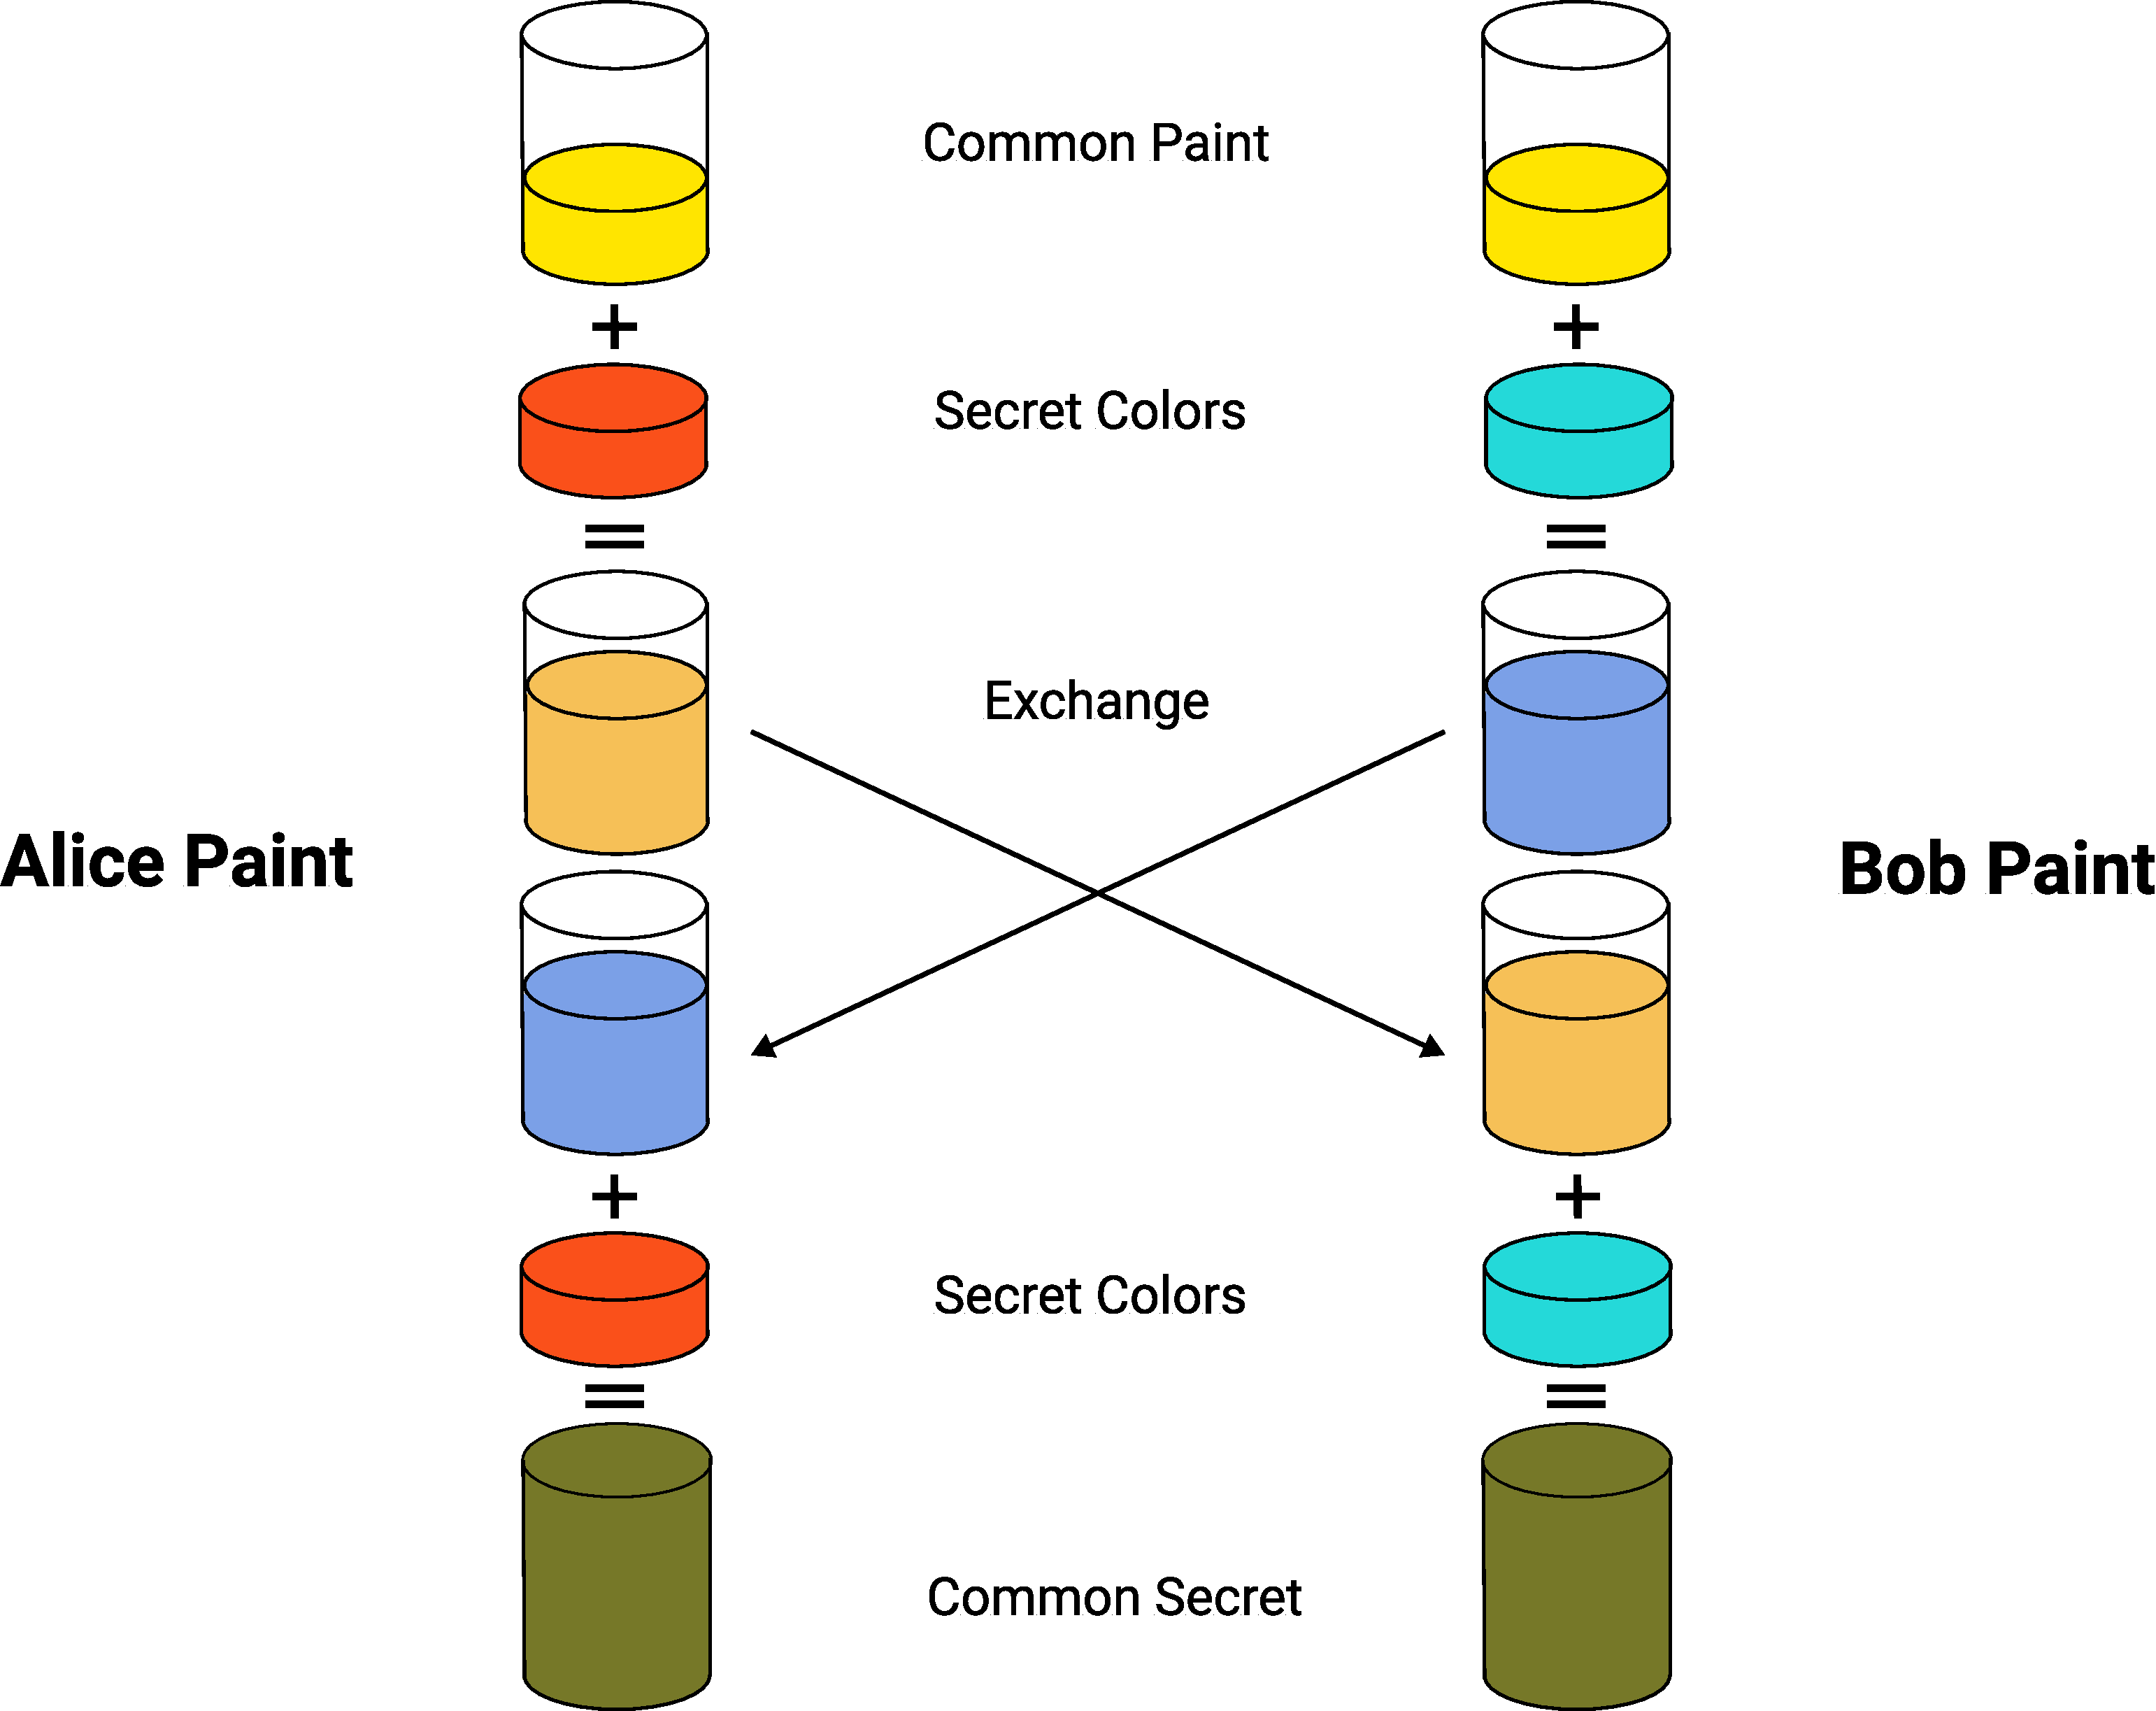
\includegraphics[width=1\textwidth]{Pictures/Diffie-Hellman}
    \caption{Illustration of the concept behind Diffie–Hellman key exchange. Source: }\label{fig:figure4}
\end{figure}
The process begins by having the two parties, Alice and Bob, publicly agree on an arbitrary starting color that does
not need to be kept secret (but should be different every time).
In this example, the color is yellow.
Each person also selects a secret color that they keep to themselves – in this case, red and blue-green.
The crucial part of the process is that Alice and Bob each mix their own secret color together with their mutually
shared color, resulting in orange-tan and light-blue mixtures respectively, and then publicly exchange the two mixed colors.
Finally, each of them mixes the color they received from the partner with their own private color.
The result is a final color mixture (yellow-brown in this case) that is identical to the partner's final color mixture.
If a third party listened to the exchange, it would only know the common color (yellow) and the first mixed colors
(orange-tan and light-blue), but it would be difficult for this party to determine the final secret color (yellow-brown).
Bringing the analogy back to a real-life exchange using large numbers rather than colors, this determination is
computationally expensive.
It is impossible to compute in a practical amount of time even for modern supercomputers.

The simplest and the original implementation of the protocol uses the multiplicative group of integers modulo $P$,
where $P$ is prime, and the generator $G$ which is a primitive root modulo $P$.
These two values are chosen in this way to ensure that the resulting shared secret can take on any value from $1$ to $P-1$.
Here is an example of the protocol
\begin{enumerate}
    \item Given modulus $P$ and generator $G$.
    \item Alice chooses her secret $a$.
    \item Alice sends to Bob $A, \; A = G^a \bmod P$.
    \item Bob chooses his secret $b$.
    \item Bob sends to Alice $B, \; B = G^b \bmod P$.
    \item Alice computes common secret $s, \; s = B^a \bmod P = (G^b \bmod P)^a \bmod P$.
    \item Bob computes common secret $s, \; s = A^b \bmod P = (G^a \bmod P)^b \bmod P$.
    \item Alice and Bob have arrived to the same value
    \[
        A^b \bmod P = G^{ab} \bmod P = G^{ba} \bmod P = B^a \bmod P,
    \]
    more specially,
    \[
        (G^a \bmod P)^b \bmod P = (G^b \bmod P)^a
    \]
\end{enumerate}
However, to reach a satisfactory level of security through DH key exchange a few rules have to be satisfied.
More precisely, Diffie-Hellman works in a multiplicative subgroup of integers modulo a given prime $p$.
To do some DH, you use some DH parameters which are:
\begin{itemize}
    \item p -- a big prime, called the "modulus"
    \item q -- a divisor of $p-1$, called the "subgroup order".
    \item g -- an integer modulo $p$ of order $q$, this means that the smallest integer $k > 0$ such that
    $g^k = 1 \bmod p$ is $k = q$.
\end{itemize}
For DH to be safe, you need the following:

\begin{itemize}
    \item Prime $p$ must defeat attempt at discrete logarithm through Index Calculus.
    This means that $p$ must be large enough, and also must not have any "special structure"
    such as being very close to a power of 2, because such structures allow for improvements in Index Calculus.
    It so happens that size requirements for DH are about the same as the size requirements for RSA,
    though the underlying reason for that is intricate and partly coincidental.
    So, basically, use a random $p$ of 2048 bits, and you will be fine.
    \item Number $q$ should be prime or have a prime divisor whose size is enough to defeat generic algorithms for
    discrete logarithm.
    If the size (in bits) of the largest prime divisor of $q$ is $z$, then generic algorithms have a cost in $2^{z/2}$.
    For best results, arrange for $q$ to be a prime of 256 bits or more.
    \item Systems that use the parameters to perform a DH key exchange must generate a random integer
    between $1$ and $q-1$ uniformly, using a cryptographically strong source of randomness, of course.
    If $q$ is prime and larger than 256 bits, it suffices to choose a 256-bit random value
    to achieve 128-bit of security.
    However, if $q$ is not prime, things are more complex: if $q$ has size $r$ bits,
    and the largest prime divisor of $q$ has size $e$ bits, and $e \geq 256$,
    then one may choose a random value $x$ of size $r-(e-256)$
    bits to get the usual "128-bit security".
    \item When $p$ is a so-called "safe prime", then $p = 2r+1$ for a prime $r$, so for any generator $g$ that is
    not $1$ or $p-1$, the order of $g$ will be either $r$ or $2r$, so it suffices to generate DH secret keys
    $x$ as random 257-bit values.
    The "safe primes" are not actually any safer than other primes,
    except for that point: they tolerate the choice of relatively small DH secret keys for any generator.
    \item Last but not least, DH is a key exchange algorithm that does not,
    inherently, provide authentication or confidentiality.
    DH is "safe" only when used within a protocol that uses DH and other algorithms with proper
    integration to achieve such sought after characteristics as data confidentiality and integrity.
\end{itemize}

Speaking of which, some (many) SSL/TLS implementations did things improperly, in that they
gladly accepted to do DH with weak parameters, in particular a 512-bit modulus.
The protocol itself is suboptimal in its handling of DH because the \texttt{ServerKeyExchange}
message allows the server to send the DH parameters $p$ and $g$ to the client, but not $q$,
leaving the client a bit in the dark.
Thus, the client must either "play safe" and generate its key in the full $1, \;\dots,\; p-1$ range,
or try to use a shorter exponent (say, 256 bits, not 2048) for a reduced computational cost,
but possibly at risk of weakness in case the subgroup order $q$ is not prime.
A better design would have allowed the server to send the value of $q$ and the size of the
biggest prime divisor of $q$.
In that respect, the ECDHE cipher suites of SSL/TLS (DH translated to elliptic curves)
have a better design.

For a practical answer if you are configuring your SSL/TLS server:
you should use a modulus of at least 2048-bit, and a generator $g$ such that the order
of $g$ is a prime $q$ of at least 256 bits;
alternatively, you may use a modulus $p$ which
is a "safe prime", the order of $g$ will then be either a very big prime, or twice
a very big prime, which is almost as good.
Some people feel safer when they generate their DH parameters
"themselves" instead of reusing existing values;
if that's what it takes
to allow you to sleep at night, then do it.

%\subsection{Secrecy Chart}\label{subsec:secrecy-chart}
%The chart below depicts who knows what, again with non-secret values in \textcolor{blue}{blue}, and secret values in \textcolor{red}{red}.
%Here Eve is an eavesdropper – she watches what is sent between Alice and Bob, but she does not alter the contents of their communications.
%\begin{itemize}
%    \item \textcolor{blue}{g} = public (prime) base, known to Alice, Bob, and Eve. $\textcolor{blue}{g = 5}$
%    \item \textcolor{blue}{p} = public (prime) modulus, known to Alice, Bob, and Eve. $\textcolor{blue}{p = 23}$
%    \item \textcolor{red}{a} = Alice's private key, known only to Alice. $\textcolor{red}{a = 6}$
%    \item \textcolor{red}{b} = Bob's private key known only to Bob. $\textcolor{red}{b = 15}$
%    \item \textcolor{blue}{A} = Alice's public key, known to Alice, Bob, and Eve. $\textcolor{blue}{A = g}^{\textcolor{red}{a}} \, mod \, \textcolor{blue}{p = 8}$
%    \item \textcolor{blue}{B} = Bob's public key, known to Alice, Bob, and Eve. $\textcolor{blue}{B = g}^{\textcolor{red}{a}} \, mod \, \textcolor{blue}{p = 8}$
%\end{itemize}
%\begin{center}
%    \begin{table}
%        \begin{tabular}{|c|c|c|c|c|c|}
%            \hline
%            \multicolumn{2}{|c|}{Alice} & \multicolumn{2}{c|}{Bob} & \multicolumn{2}{c|}{Eve}
%            \cr \hline
%            known & unknown & known & unknown & known & unknown
%            \cr \hline
%            $\textcolor{blue}{p = 23}$ & & $\textcolor{blue}{p = 23}$  & & $\textcolor{blue}{p = 23}$ &
%            \cr \hline
%            $\textcolor{blue}{g = 5}$ & & $\textcolor{blue}{g = 5}$ & & $\textcolor{blue}{g = 5}$ &
%            \cr \hline
%            $\textcolor{red}{a = 6}$ & $\textcolor{red}{b}$ & $\textcolor{red}{b = 15}$ & $\textcolor{red}{a}$ & & $\textcolor{red}{a, b}$
%            \cr \hline
%            $\textcolor{blue}{A = 5}^{\textcolor{red}{a}} \, mod \, \textcolor{blue}{23}$ & & $\textcolor{blue}{B = 5}^{\textcolor{red}{b}} \, mod \, \textcolor{blue}{23}$ & & &
%            \cr \hline
%            $\textcolor{blue}{A = 5}^{\textcolor{red}{6}} \, mod \, \textcolor{blue}{23} = \textcolor{blue}{8}$ & & $\textcolor{blue}{B = 5}^{\textcolor{red}{15}} \, mod \, \textcolor{blue}{23} = \textcolor{blue}{19}$ & & &
%            \cr \hline
%            $\textbf{\textcolor{blue}{B}} = \textbf{\textcolor{blue}{19}}$ & & $\textbf{\textcolor{blue}{A}} = \textbf{\textcolor{blue}{8}}$ & & $\textcolor{blue}{A} = \textcolor{blue}{8}$, $\textcolor{blue}{B} = \textcolor{blue}{19}$ &
%            \cr \hline
%            $\textbf{\textcolor{red}{s}} = \textcolor{blue}{B}^{\textcolor{red}{a}} \, mod \, \textcolor{blue}{23}$ & & $\textbf{\textcolor{red}{s}} = \textcolor{blue}{A}^{\textcolor{red}{b}} \, mod \, \textcolor{blue}{23}$ & & &
%            \cr \hline
%            $\textbf{\textcolor{red}{s}} = \textcolor{blue}{19}^{\textcolor{red}{6}} \, mod \, \textcolor{blue}{23} = \textcolor{red}{2}$ & & $\textbf{\textcolor{red}{s}} = \textcolor{blue}{A}^{\textcolor{red}{b}} \, mod \, \textcolor{blue}{23} = \textcolor{red}{2}$ & & &
%            \cr \hline
%
%        \end{tabular}
%        \label{tab:table}
%    \end{table}
%\end{center}
%Now \textcolor{red}{s} is the shared secret key and it is known to both Alice and Bob, but not to Eve.
%Note that it is not helpful for Eve to compute \textcolor{blue}{AB}, which equals
%$\textcolor{blue}{g}^{\textcolor{red}{a} + \textcolor{red}{b}} \, mod \, \textcolor{blue}{p}$.
%Note that it should be difficult for Alice to solve for Bob's private key or for Bob to solve for Alice's private key.
%If it is not difficult for Alice to solve for Bob's private key (or vice versa), Eve may simply substitute her own
%private / public key pair, plug Bob's public key into her private key, produce a fake shared secret key, and solve for
%Bob's private key (and use that to solve for the shared secret key.
%Eve may attempt to choose a public / private key pair that will make it easy for her to solve for Bob's private key).

\begin{figure}[H]
    \centering
    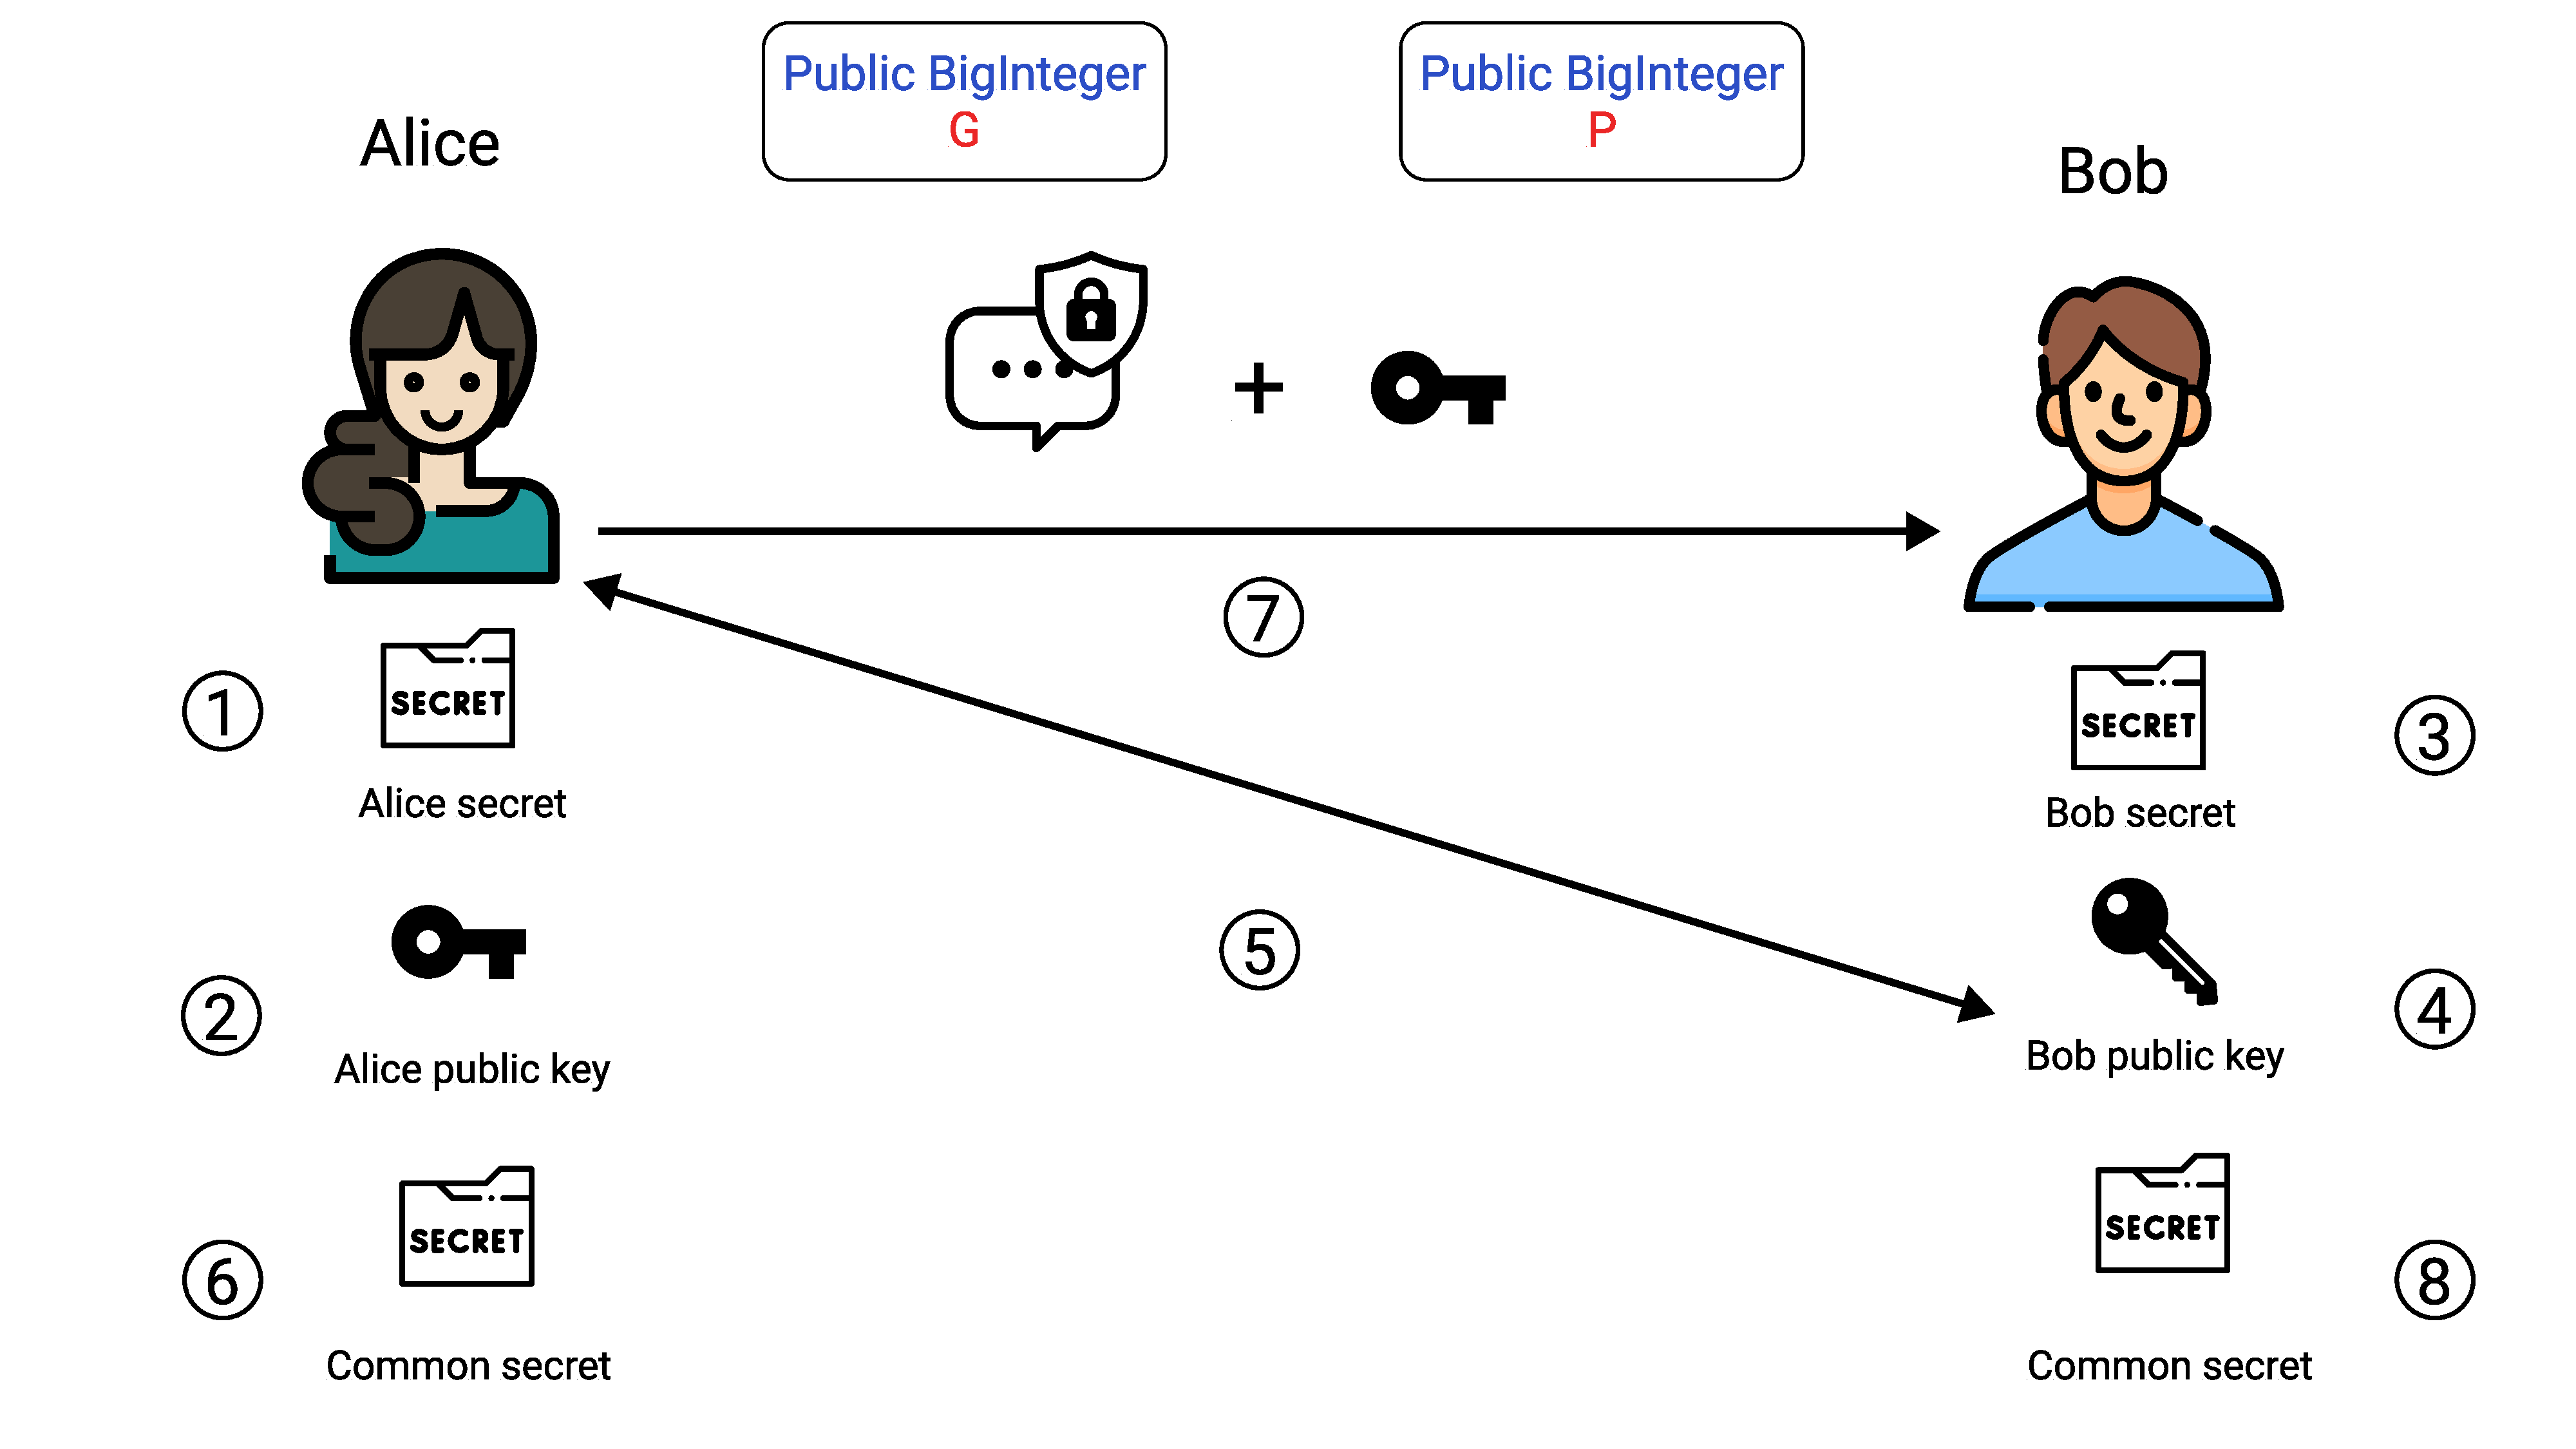
\includegraphics[width=1\textwidth]{Pictures/Key_Exchange}
    \caption{Secret chat encryption concept diagram. Source: }\label{fig:figure7}
\end{figure}
Assume that Alice wants to write a secret message to the Bob.
The secret chat encryption implemented as follows
\begin{enumerate}
    \item Given two public constants: $P, G$.
    \item Alice generates her secret $a$.
    \item Alice generates public key $A$ as $A=G^a \bmod P$ and shares it public.
    \item Bob generates his secret $b$.
    \item Bob generates public key $B$ as $B=G^b \bmod P$ and shares it public.
    \item Alice reads Bob's public key $B$.
    \item Alice calculates Common secret $s$ as $s = B^a \bmod P$.
    \item Alice encrypts message using AES256 algorithm, then sends it to Bob along her public key $A$.
    \item Bob calculates Common secret $s$ as $s = A^b \bmod P$ and decrypts message from Alice.
\end{enumerate}
Although, DH fits the key exchange concerns fine, the secret might be shared via RSA approach as well.
We discuss it in next section.

%----------------------------------------------------------------------------------------
%	BIBLIOGRAPHY
%----------------------------------------------------------------------------------------

    \printbibliography[heading=bibintoc]

%----------------------------------------------------------------------------------------

%----------------------------------------------------------------------------------------
%	THESIS CONTENT - APPENDICES
%----------------------------------------------------------------------------------------

    \appendix % Cue to tell LaTeX that the following "chapters" are Appendices

% Include the appendices of the thesis as separate files from the Appendices folder
% Uncomment the lines as you write the Appendices

    %\chapter{Web API Documentation}\label{ch:web-api-documentation}


\section{Auth}\label{sec:auth}
\begin{itemize}
    %% Register Endpoint
    \item \textbf{Endpoint}: /api/auth/register
    \begin{itemize}
        \item \textbf{Description}: Registers user in a messenger
        \item \textbf{Request type}: POST
        \item \textbf{Request body}:
        \begin{spverbatim}
        {
            "phoneNumber": "string",
            "email": "string",
            "displayName": "string",
            "password": "string",
            "verificationMethod": number,
            "termsAccepted": boolean
        }
        \end{spverbatim}
        \item  \textbf{Response example}:
        \begin{itemize}
            \item \textbf{200 Success}:
            \begin{spverbatim}
            {
                "message": "SUCCESS",
                "success": true
            }
            \end{spverbatim}
            \item \textbf{400 Bad Request}:
            \begin{spverbatim}
            {
                "errorMessage": "string",
                "errorDetails": "string",
                "statusCode": 0,
                "success": true
            }
            \end{spverbatim}
            \item \textbf{409 Conflict}:
            \begin{spverbatim}
            {
                "errorMessage": "string",
                "errorDetails": "string",
                "statusCode": 0,
                "success": true
            }
            \end{spverbatim}
        \end{itemize}
        \item \textbf{Response messages}:
        \begin{enumerate}
            \item Success.
            \item User already registered.
            \item Weak password.
            \item Invalid email.
            \item Invalid verification method.
            \item Invalid display name.
            \item Phone occupied.
        \end{enumerate}
    \end{itemize}
    %% Register Endpoint

    %% Verify Email Endpoint
    \item \textbf{Endpoint}: api/auth/verify-email
    \begin{itemize}
        \item \textbf{Description}: Sends verification request.
        User receives confirmation link via email.
        \item \textbf{Request type}: POST
        \item \textbf{Request body}:
        \begin{spverbatim}
        {
            "email": "string",
            "userId": "string"
        }
        \end{spverbatim}
        \item  \textbf{Response example}:
        \begin{itemize}
            \item \textbf{200 Success}:
            \begin{spverbatim}
            {
                "message": "SUCCESS",
                "success": true
            }
            \end{spverbatim}
            \item \textbf{400 Bad Request}:
            \begin{spverbatim}
            {
                "errorMessage": "string",
                "errorDetails": "string",
                "statusCode": 0,
                "success": true
            }
            \end{spverbatim}
            \item \textbf{409 Conflict}:
            \begin{spverbatim}
            {
                "errorMessage": "string",
                "errorDetails": "string",
                "statusCode": 0,
                "success": true
            }
            \end{spverbatim}
        \end{itemize}
        \item \textbf{Response messages}:
        \begin{enumerate}
            \item Success.
            \item User already registered.
            \item Weak password.
            \item Invalid email.
            \item Invalid verification method.
            \item Invalid display name.
            \item Phone occupied.
        \end{enumerate}
        \item \textbf{Response messages}:
        \begin{enumerate}
            \item Success.
            \item Invalid user id.
            \item Email already verified.
        \end{enumerate}
    \end{itemize}
    %% Verify Email Endpoint

    %% Verify Phone Endpoint
    \item \textbf{Endpoint}: api/auth/verify-phone
    \begin{itemize}
        \item \textbf{Description}: Sends SMS to user phone.
        \item \textbf{Request type}: POST
        \item \textbf{Request body}:
        \begin{spverbatim}
        {
            "confirmationCode": 0,
            "userId": "string"
        }
        \end{spverbatim}
        \item  \textbf{Response example}:
        \begin{itemize}
            \item \textbf{200 Success}:
            \begin{spverbatim}
            {
                "message": "SUCCESS",
                "success": true
            }
            \end{spverbatim}
            \item \textbf{400 Bad Request}:
            \begin{spverbatim}
            {
                "errorMessage": "string",
                "errorDetails": "string",
                "statusCode": 0,
                "success": true
            }
            \end{spverbatim}
            \item \textbf{409 Conflict}:
            \begin{spverbatim}
            {
                "errorMessage": "string",
                "errorDetails": "string",
                "statusCode": 0,
                "success": true
            }
            \end{spverbatim}
        \end{itemize}
        \item \textbf{Response messages}:
        \begin{enumerate}
            \item Success.
            \item Invalid or expired.
            \item Phone already verified
        \end{enumerate}
    \end{itemize}
    %% Verify Phone Endpoint

    %% Login Endpoint
    \item \textbf{Endpoint}: api/auth/login
    \begin{itemize}
        \item \textbf{Description}: Performs login to the messenger.
        \item \textbf{Request type}: POST
        \item \textbf{Request body}:
        \begin{spverbatim}
        {
            "email": "string",
            "password": "string"
        }
        \end{spverbatim}
        \item \textbf{Response example}:
        \begin{itemize}
            \item \textbf{200 Success}:
            \begin{spverbatim}
            {
                "refreshTokenId": "string",
                "accessToken": "string",
                "message": "string",
                "success": true
            }
            \end{spverbatim}
            \item \textbf{400 Bad Request}:

            \begin{spverbatim}
            {
                "errorMessage": "string",
                "errorDetails": "string",
                "statusCode": 0,
                "success": true
            }
            \end{spverbatim}
            \item \textbf{409 Conflict}:
            \begin{spverbatim}
            {
                "errorMessage": "string",
                "errorDetails": "string",
                "statusCode": 0,
                "success": true
            }
            \end{spverbatim}
        \end{itemize}
        \item \textbf{Response messages}:
        \begin{enumerate}
            \item Success.
            \item Invalid credentials.
        \end{enumerate}
    \end{itemize}
    %% Login Endpoint


    %% Refresh Token Endpoint
    \item \textbf{Endpoint}: api/auth/refresh-token
    \begin{itemize}
        \item \textbf{Description}: Refreshes user's existing refresh token and access token.
        \item \textbf{Request type}: POST
        \item \textbf{Request body}:
        \begin{spverbatim}
        {
            "refreshTokenId": "string"
        }
        \end{spverbatim}
        \item  \textbf{Response example}:
        \begin{itemize}
            \item \textbf{200 Success}:
            \begin{spverbatim}
            {
                "refreshTokenId": "string",
                "accessToken": "string",
                "message": "string",
                "success": true
            }
            \end{spverbatim}
            \item \textbf{400 Bad Request}:
            \begin{spverbatim}
            {
                "errorMessage": "string",
                "errorDetails": "string",
                "statusCode": 0,
                "success": true
            }
            \end{spverbatim}
            \item \textbf{409 Conflict}:
            \begin{spverbatim}
            {
                "errorMessage": "string",
                "errorDetails": "string",
                "statusCode": 0,
                "success": true
            }
            \end{spverbatim}
        \end{itemize}
        \item \textbf{Response messages}:
        \begin{enumerate}
            \item Success.
            \item Invalid or empty refresh token.
        \end{enumerate}
    \end{itemize}
    %% Refresh Token Endpoint

    %% Logout Endpoint
    \item \textbf{Endpoint}: api/auth/logout
    \begin{itemize}
        \item \textbf{Description}: Logs out from current device.
        \item \textbf{Request type}: POST
        \item \textbf{Request body}:
        \begin{spverbatim}
        {
            "refreshTokenId": "string"
        }
        \end{spverbatim}
        \item \textbf{Response example}:
        \begin{itemize}
            \item \textbf{200 Success}:
            \begin{spverbatim}
            {
                "message": "SUCCESS",
                "success": true
            }
            \end{spverbatim}
            \item \textbf{400 Bad Request}:
            \begin{spverbatim}
            {
                "errorMessage": "string",
                "errorDetails": "string",
                "statusCode": 0,
                "success": true
            }
            \end{spverbatim}
            \item \textbf{409 Conflict}:
            \begin{spverbatim}
            {
                "errorMessage": "string",
                "errorDetails": "string",
                "statusCode": 0,
                "success": true
            }
            \end{spverbatim}
        \end{itemize}
        \item \textbf{Response messages}:
        \begin{enumerate}
            \item Success.
            \item User not found.
            \item Invalid or empty refresh token.
        \end{enumerate}
    \end{itemize}
    %% Logout Endpoint

    %% Logout All Endpoint
    \item \textbf{Endpoint}: api/auth/logout-all
    \begin{itemize}
        \item \textbf{Description}: Logs out from all devices.
        \item \textbf{Request type}: POST
        \item \textbf{Request body}:
        \begin{spverbatim}
        {
            "refreshTokenId": "string"
        }
        \end{spverbatim}
        \item  \textbf{Response example}:
        \begin{itemize}
            \item \textbf{200 Success}:
            \begin{spverbatim}
            {
                "message": "SUCCESS",
                "success": true
            }
            \end{spverbatim}
            \item \textbf{400 Bad Request}:
            \begin{spverbatim}
            {
                "errorMessage": "string",
                "errorDetails": "string",
                "statusCode": 0,
                "success": true
            }
            \end{spverbatim}
            \item \textbf{409 Conflict}:
            \begin{spverbatim}
            {
                "errorMessage": "string",
                "errorDetails": "string",
                "statusCode": 0,
                "success": true
            }
            \end{spverbatim}
        \end{itemize}
    \end{itemize}
    %% Logout All Endpoint

\end{itemize}


\section{Chats}\label{sec:chats}
\begin{itemize}
    %% Get Chats Endpoint
    \item \textbf{Endpoint}: api/chats
    \begin{itemize}
        \item \textbf{Description}: Returns list of all user's chats.
        \item \textbf{Request type}: GET
        \item \textbf{Response example}:
        \textbf{200 Success}:
        \begin{spverbatim}
        {
            "chats": [
                {
                "chatId": "string",
                "title": "string",
                "image": "string",
                "lastMessageAuthor": "string",
                "lastMessage": "string",
                "lastMessageAt": "string",
                "membersCount": 0,
                "isMember": true
            }
            ],
            "message": "string",
            "success": true
        }
        \end{spverbatim}
        \textbf{400 Bad Request}:
        \begin{spverbatim}
        {
            "errorMessage": "string",
            "errorDetails": "string",
            "statusCode": 0,
            "success": true
        }
        \end{spverbatim}
        \textbf{409 Conflict}:
        \begin{spverbatim}
        {
            "errorMessage": "string",
            "errorDetails": "string",
            "statusCode": 0,
            "success": true
        }
        \end{spverbatim}
        \item \textbf{Response messages}:
        \begin{enumerate}
            \item Success.
            \item User not found.
        \end{enumerate}
    \end{itemize}
    %% Get Chats Endpoint

    %% Create Group Endpoint
    \item \textbf{Endpoint}: api/chats/group
    \begin{itemize}
        \item \textbf{Description}: Creates new group of specified type.
        \item \textbf{Request type}: POST
        \item \textbf{Request body}:
        \begin{spverbatim}
        {
            "groupType": 1
            "groupTitle": "string"
        }
        \end{spverbatim}
        \item \textbf{Chat types}:
        \begin{enumerate}
            \item DirectChat -- Chat between two people
            \item PrivateChannel -- Channel that can be joined only via invite link from owner or one of the members
            \item PublicChannel -- Channel that can be joined and messaged by anyone, unless person is not in blacklist
            \item ReadOnlyChannel -- Channel that can be joined by anyone, but any member except owner or moderator cannot send messages there
        \end{enumerate}
        \item \textbf{Response example}:
        \textbf{200 Success}:
        \begin{spverbatim}
        {
            "chatId": "string",
            "message": "string",
            "success": true
        }
        \end{spverbatim}
        \textbf{400 Bad Request}:
        \begin{spverbatim}
        {
            "errorMessage": "string",
            "errorDetails": "string",
            "statusCode": 0,
            "success": true
        }
        \end{spverbatim}
        \textbf{409 Conflict}:
        \begin{spverbatim}
        {
            "errorMessage": "string",
            "errorDetails": "string",
            "statusCode": 0,
            "success": true
        }
        \end{spverbatim}
        \item \textbf{Response messages}:
        \begin{enumerate}
            \item Success.
            \item User not found.
        \end{enumerate}
    \end{itemize}
    %% Create Group Endpoint

    %% Create Direct Chat Endpoint
    \item \textbf{Endpoint}: api/chats/direct-chat
    \begin{itemize}
        \item \textbf{Description}: Creates new group of specified type.
        \item \textbf{Request type}: POST
        \item \textbf{Request body}:
        \begin{spverbatim}
        {
            "partnerId": "string"
        }
        \end{spverbatim}
        \item \textbf{Response example}:
        \textbf{200 Success}:
        \begin{spverbatim}
        {
            "chatId": "string",
            "message": "string",
            "success": true
        }
        \end{spverbatim}
        \textbf{400 Bad Request}:
        \begin{spverbatim}
        {
            "errorMessage": "string",
            "errorDetails": "string",
            "statusCode": 0,
            "success": true
        }
        \end{spverbatim}
        \textbf{409 Conflict}:
        \begin{spverbatim}
        {
            "errorMessage": "string",
            "errorDetails": "string",
            "statusCode": 0,
            "success": true
        }
        \end{spverbatim}
        \item \textbf{Response messages}:
        \begin{enumerate}
            \item Success.
            \item User not found.
        \end{enumerate}
    \end{itemize}
    %% Create Direct Chat Endpoint

    %% Group Join Endpoint
    \item \textbf{Endpoint}: api/chats/group/join/\{chatId\}
    \begin{itemize}
        \item \textbf{Description}: Creates new group of specified type.
        \item \textbf{Request type}: POST
        \item \textbf{Request example}:
        \begin{spverbatim}
        {
            "chatId": "string"
        }
        \end{spverbatim}
        \item \textbf{Response example}:
        \textbf{200 Success}:
        \begin{spverbatim}
        {
            "chatId": "string",
            "message": "string",
            "success": true
        }
        \end{spverbatim}
        \textbf{400 Bad Request}:
        \begin{spverbatim}
        {
            "errorMessage": "string",
            "errorDetails": "string",
            "statusCode": 0,
            "success": true
        }
        \end{spverbatim}
        \textbf{409 Conflict}:
        \begin{spverbatim}
        {
            "errorMessage": "string",
            "errorDetails": "string",
            "statusCode": 0,
            "success": true
        }
        \end{spverbatim}
        \item \textbf{Response messages}:
        \begin{enumerate}
            \item Success.
            \item Group not found.
        \end{enumerate}
    \end{itemize}
    %% Group Join Endpoint

    %% Search Chat Endpoint
    \item \textbf{Endpoint}: api/chats/search
    \begin{itemize}
        \item \textbf{Description}: Searches chats by display name.
        \item \textbf{Request type}: GET
        \item \textbf{Parameters}:
        \begin{enumerate}
            \item displayName (required)
        \end{enumerate}
        \item \textbf{Response example}:
        \textbf{200 Success}:
        \begin{spverbatim}
        {
            "chats": [
                {
                "chatId": "string",
                "title": "string",
                "image": "string",
                "lastMessageAuthor": "string",
                "lastMessage": "string",
                "lastMessageAt": "string",
                "membersCount": 0,
                "isMember": true
            }
            ],
            "message": "string",
            "success": true
        }
        \end{spverbatim}
        \textbf{400 Bad Request}:
        \begin{spverbatim}
        {
            "errorMessage": "string",
            "errorDetails": "string",
            "statusCode": 0,
            "success": true
        }
        \end{spverbatim}
        \textbf{409 Conflict}:
        \begin{spverbatim}
        {
            "errorMessage": "string",
            "errorDetails": "string",
            "statusCode": 0,
            "success": true
        }
        \end{spverbatim}
        \item \textbf{Response messages}:
        \begin{enumerate}
            \item Success.
            \item Unauthorized.
        \end{enumerate}
    \end{itemize}
    %% Search Chat Endpoint

\end{itemize}


\section{Messages}\label{sec:messages}
\begin{itemize}
    %% Get Chat Messages Endpoint
    \item \textbf{Endpoint}: /api/messages/\{chatId\}
    \begin{itemize}
        \item \textbf{Description}: Returns chat including messages by chat id.
        \item \textbf{Request type}: GET
        \item \textbf{Parameters}:
        \begin{enumerate}
            \item Chat id (required).
        \end{enumerate}
        \item \textbf{Response example}:
        \begin{itemize}
            \item \textbf{200 Success}:
            \begin{spverbatim}
            {
                "messages": [
                    {
                        "userDisplayName": "string",
                        "messageText": "string",
                        "sentAt": "string",
                        "editedAt": "string",
                        "self": true
                    }
                ],
                "message": "string",
                "success": true
            }
            \end{spverbatim}
            \item \textbf{400 Bad Request}:
            \begin{spverbatim}
            {
                "errorMessage": "string",
                "errorDetails": "string",
                "statusCode": 0,
                "success": true
            }
            \end{spverbatim}
            \item \textbf{409 Conflict}:
            \begin{spverbatim}
            {
                "errorMessage": "string",
                "errorDetails": "string",
                "statusCode": 0,
                "success": true
            }
            \end{spverbatim}
        \end{itemize}
        \item \textbf{Response messages}:
        \begin{enumerate}
            \item Success.
            \item User not found.
        \end{enumerate}
    \end{itemize}
    %% Get Chat Messages Endpoint

    %% Send Message Endpoint
    \item \textbf{Endpoint}: /api/messages
    \begin{itemize}
        \item \textbf{Description}: Sends message to particular chat
        \item \textbf{Request type}: POST
        \item \textbf{Request body}:
        \begin{spverbatim}
        {
            "messageId": "string",
            "message": "string",
            "success": true
        }
        \end{spverbatim}
        \item \textbf{Response example}:
        \begin{itemize}
            \item \textbf{200 Success}:
            \begin{spverbatim}
            {
                "message": "SUCCESS",
                "success": true
            }
            \end{spverbatim}
            \item \textbf{400 Bad Request}:
            \begin{spverbatim}
            {
                "errorMessage": "string",
                "errorDetails": "string",
                "statusCode": 0,
                "success": true
            }
            \end{spverbatim}
            \item \textbf{409 Conflict}:
            \begin{spverbatim}
            {
                "errorMessage": "string",
                "errorDetails": "string",
                "statusCode": 0,
                "success": true
            }
            \end{spverbatim}
        \end{itemize}
        \item \textbf{Response messages}:
        \begin{enumerate}
            \item Success.
            \item User not found.
        \end{enumerate}
    \end{itemize}
    %% Send Message Endpoint

    %% Edit Message Endpoint
    \item \textbf{Endpoint}: /api/messages
    \begin{itemize}
        \item \textbf{Description}: Updates particular message
        \item \textbf{Request type}: PUT
        \item \textbf{Request body}:
        \begin{spverbatim}
        {
            "messageId": "string",
            "modifiedText": "string"
        }
        \end{spverbatim}
        \item \textbf{Response example}:
        \begin{itemize}
            \item \textbf{200 Success}:
            \begin{spverbatim}
            {
                "message": "SUCCESS",
                "success": true
            }
            \end{spverbatim}
            \item \textbf{400 Bad Request}:
            \begin{spverbatim}
            {
                "errorMessage": "string",
                "errorDetails": "string",
                "statusCode": 0,
                "success": true
            }
            \end{spverbatim}
            \item \textbf{409 Conflict}:
            \begin{spverbatim}
            {
                "errorMessage": "string",
                "errorDetails": "string",
                "statusCode": 0,
                "success": true
            }
            \end{spverbatim}
        \end{itemize}
        \item \textbf{Response messages}:
        \begin{enumerate}
            \item Success.
            \item User not found.
        \end{enumerate}
    \end{itemize}
    %% Edit Message Endpoint

    %% Delete Message Endpoint
    \item \textbf{Endpoint}: /api/messages
    \begin{itemize}
        \item \textbf{Description}: Deletes particular message
        \item \textbf{Request type}: DELETE
        \item \textbf{Request body}:
        \begin{spverbatim}
        {
            "messageId": "string"
        }
        \end{spverbatim}
        \item \textbf{Response example}:
        \begin{itemize}
            \item \textbf{200 Success}:
            \begin{spverbatim}
            {
                "message": "SUCCESS",
                "success": true
            }
            \end{spverbatim}
            \item \textbf{400 Bad Request}:
            \begin{spverbatim}
            {
                "errorMessage": "string",
                "errorDetails": "string",
                "statusCode": 0,
                "success": true
            }
            \end{spverbatim}
            \item \textbf{409 Conflict}:
            \begin{spverbatim}
            {
                "errorMessage": "string",
                "errorDetails": "string",
                "statusCode": 0,
                "success": true
            }
            \end{spverbatim}
        \end{itemize}
        \item \textbf{Response messages}:
        \begin{enumerate}
            \item Success.
            \item User not found.
        \end{enumerate}
    \end{itemize}
    %% Delete Message Endpoint
\end{itemize}


\section{User}\label{sec:user}
\begin{itemize}
    %% Get User Endpoint
    \item \textbf{Endpoint}: /api/users/\{userId\}
    \begin{itemize}
        \item \textbf{Description}: Returns information about particular user by user ID
        \item \textbf{Request type}: GET
        \item \textbf{Parameters}:
        \begin{enumerate}
            \item User ID (required).
        \end{enumerate}
        \item \textbf{Response example}:
        \textbf{200 Success}:
        \begin{spverbatim}
        {
            "message": "string",
            "success": true
        }
        \end{spverbatim}
        \textbf{400 Bad Request}:
        \begin{spverbatim}
        {
            "errorMessage": "string",
            "errorDetails": "string",
            "statusCode": 0,
            "success": true
        }
        \end{spverbatim}
        \textbf{409 Conflict}:
        \begin{spverbatim}
        {
            "errorMessage": "string",
            "errorDetails": "string",
            "statusCode": 0,
            "success": true
        }
        \end{spverbatim}
        \item \textbf{Response messages}:
        \begin{enumerate}
            \item Success.
            \item User not found.
        \end{enumerate}
    \end{itemize}
    %% Get User Endpoint
    %% Get Current User Endpoint
    \item \textbf{Endpoint}: /api/users
    \begin{itemize}
        \item \textbf{Description}: Returns information about current user logged in system
        \item \textbf{Request type}: GET
        \item \textbf{Response example}:
        \textbf{200 Success}:
        \begin{spverbatim}
        {
            "user": {
            "username": "string",
            "displayName": "string",
            "bio": "string",
            "image": "string"
        },
            "message": "string",
            "success": true
        }
        \end{spverbatim}
        \textbf{400 Bad Request}:
        \begin{spverbatim}
        {
            "errorMessage": "string",
            "errorDetails": "string",
            "statusCode": 0,
            "success": true
        }
        \end{spverbatim}
        \textbf{409 Conflict}:
        \begin{spverbatim}
        {
            "errorMessage": "string",
            "errorDetails": "string",
            "statusCode": 0,
            "success": true
        }
        \end{spverbatim}
        \item \textbf{Response messages}:
        \begin{enumerate}
            \item Success.
            \item User not found.
        \end{enumerate}
    \end{itemize}
    %% Get Loged User Endpoint
    %% Search User Endpoint
    \item \textbf{Endpoint}: /api/users/search
    \begin{itemize}
        \item \textbf{Description}: Searches user by display name
        \item \textbf{Request type}: GET
        \item \textbf{Parameters}:
        \begin{enumerate}
            \item displayName (required)
        \end{enumerate}
        \item \textbf{Response example}:
        \textbf{200 Success}:
        \begin{spverbatim}
        {
            "user": {
            "username": "string",
            "displayName": "string",
            "bio": "string",
            "image": "string"
        },
            "message": "string",
            "success": true
        }
        \end{spverbatim}
        \textbf{400 Bad Request}:
        \begin{spverbatim}
        {
            "errorMessage": "string",
            "errorDetails": "string",
            "statusCode": 0,
            "success": true
        }
        \end{spverbatim}
        \textbf{409 Conflict}:
        \begin{spverbatim}
        {
            "errorMessage": "string",
            "errorDetails": "string",
            "statusCode": 0,
            "success": true
        }
        \end{spverbatim}
        \item \textbf{Response messages}:
        \begin{enumerate}
            \item Success.
            \item User not found.
        \end{enumerate}
    \end{itemize}
    %% Search User Endpoint
\end{itemize}


\section{Contacts}\label{sec:contacts}
\begin{itemize}
    %% Add Contact Endpoint
    \item \textbf{Endpoint}: /api/contacts
    \begin{itemize}
        \item \textbf{Description}: Adds new contact
        \item \textbf{Request type}: POST
        \item \textbf{Request body}:
        \begin{spverbatim}
        {
            "contactId": "string"
        }
        \end{spverbatim}
        \item \textbf{Response example}:
        \textbf{200 Success}:
        \begin{spverbatim}
        {
            "message": "string",
            "success": true
        }
        \end{spverbatim}
        \textbf{400 Bad Request}:
        \begin{spverbatim}
        {
            "errorMessage": "string",
            "errorDetails": "string",
            "statusCode": 0,
            "success": true
        }
        \end{spverbatim}
        \textbf{409 Conflict}:
        \begin{spverbatim}
        {
            "errorMessage": "string",
            "errorDetails": "string",
            "statusCode": 0,
            "success": true
        }
        \end{spverbatim}
        \item \textbf{Response messages}:
        \begin{enumerate}
            \item Success.
            \item User not found.
        \end{enumerate}
    \end{itemize}
    %% Add Contact Endpoint
    %% Get Contacts Endpoint
    \item \textbf{Endpoint}: /api/contacts
    \begin{itemize}
        \item \textbf{Description}: Returns list of all user's contacts
        \item \textbf{Request type}: GET
        \item \textbf{Response example}:
        \textbf{200 Success}:
        \begin{spverbatim}
        {
            "contacts": [
                {
                "username": "string",
                "displayName": "string",
                "bio": "string",
                "image": "string"
            }
            ],
            "message": "string",
            "success": true
        }
        \end{spverbatim}
        \textbf{400 Bad Request}:
        \begin{spverbatim}
        {
            "errorMessage": "string",
            "errorDetails": "string",
            "statusCode": 0,
            "success": true
        }
        \end{spverbatim}
        \textbf{409 Conflict}:
        \begin{spverbatim}
        {
            "errorMessage": "string",
            "errorDetails": "string",
            "statusCode": 0,
            "success": true
        }
        \end{spverbatim}
        \item \textbf{Response messages}:
        \begin{enumerate}
            \item Success.
            \item User not found.
        \end{enumerate}
    \end{itemize}
    %% Get Contacts Endpoint
\end{itemize}


\section{User Information}\label{sec:user-information}
\begin{itemize}
    %% Update User Info Endpoint
    \item \textbf{Endpoint}: /api/contacts
    \begin{itemize}
        \item \textbf{Description}: Updates current user information
        \item \textbf{Request type}: PUT
        \item \textbf{Request body}:
        \begin{spverbatim}
        {
            "firstName": "string",
            "lastName": "string",
            "birthDay": "timestamp",
            "website": "string",
            "address": "string",
            "facebook": "string",
            "twitter": "string",
            "instagram": "string",
            "linkedIn": "string",
            "profilePicture": "string"
        }
        \end{spverbatim}
        \item \textbf{Response example}:
        \begin{itemize}
            \item \textbf{200 Success}:
            \begin{spverbatim}
            {
                "message": "string",
                "success": true
            }
            \end{spverbatim}
            \item \textbf{400 Bad Request}:
            \begin{spverbatim}
            {
                "errorMessage": "string",
                "errorDetails": "string",
                "statusCode": 0,
                "success": true
            }
            \end{spverbatim}
            \item \textbf{409 Conflict}:
            \begin{spverbatim}
            {
                "errorMessage": "string",
                "errorDetails": "string",
                "statusCode": 0,
                "success": true
            }
            \end{spverbatim}
        \end{itemize}
        \item \textbf{Response messages}:
        \begin{enumerate}
            \item Success.
            \item User not found.
        \end{enumerate}
    \end{itemize}
    %% Update User Info Endpoint
\end{itemize}
    \chapter{RSA Algorithm comments}\label{ch:rsa-algorithm-comments}
One way function -- is a function that is easy to compute on every input, but hard to invert given the image of a random input.
The function
\[
    m^e \bmod N \equiv C
\]
where $e, N$ are public constants is one-awy function,
because it is easy to compute $C$ given $m$, however it is hard to compute $m$ given $C$.


\section{Euler function}\label{sec:euler-function}
Given a number $N$ and its prime factorization $p_1^{e_1}\cdot p_2^{e_2} \cdots p_k^{e_k}$, then Euler's totient function
$\phi(N)$ is defined as

\[
    \phi(N) = (p_1^{e_1} - p_1^{e_1 - 1}) \cdot (p_2^{e_2} - p_2^{e_2 - 1}) \cdots (p_k^{e_k} - p_k^{e_k - 1})
\]

In particular, for positive number $M$ such that its factorization is $p1 \cdot p2$, the $\phi(M)$ is

\[
    \phi(M) = (p_1 -1) \cdot (p_2 - 1)
\]

Euler's theorem relates the modular division and exponent as follows, given number $m$, then

\[
    m^{\phi(N)} = 1 \bmod N
\]

It means that reminder of division $m^{\phi(N)}$ by $N$ is always 1.
By the equality $1^K = 1$
\[
    M^{K \cdot \phi(N)} = 1 \bmod N
\]

If we multiply both parts by $M$, we get

\[
    M \cdot M^{K \cdot \phi(N)} = M^{K \cdot \phi(N) + 1} = M \bmod N
\]


\section{How it works}\label{sec:how-it-works}
\begin{itemize}
    \item Alice defines public constants $e, N$ and shares them with Bob.
    \item Bob defines secret $m$, encrypts the message using $m$, so he has encrypted message $S$.
    \item Bob calculates $C = m^e \bmod N$.
    \item Bob sends to Alice: encrypted message $S$ and $C$.
    \item To encrypt message, Alice must calculate the $m$ having $C$, it is $m^{ed} \bmod N = m$, where $d$ is secret.
    \item To calculate $d$, Alice applies the equality $M^{K \cdot \phi(N) + 1} = M \bmod N$, therefore
    \begin{gather*}
        e \cdot d = K \cdot \phi(N) + 1\\
        d = \frac{K \cdot \phi(N) + 1}{e}\\
    \end{gather*}
    \item Alice takes prime $P2$
    \item Alice multiplies $P1$ and $P2$: $N = P1\cdot P2$
\end{itemize}
%\include{Appendices/AppendixB}
%\include{Appendices/AppendixC}
\end{document}  
